%
% Diplomarbeit mit LaTeX
% ===========================================================================
% This is part of the book "Diplomarbeit mit LaTeX".
% Copyright (c) 2002-2005 Tobias Erbsland, Andreas Nitsch
% See the file diplomarbeit_mit_latex.tex for copying conditions.
%

\chapter{Einleitung}

\section{Ausgangslage}
%\label{sec:Ausgangslage}



%\begin{quote}
%\enquote{Es gibt Alternativen zu WYSIWYG\footnote{What You See Is What You Get} Textverarbeitungen}.
%\end{quote}

Die Skriptsprache PHP gehört weltweit zu den meist genutzten serverseitigen Programmiersprachen. Im August 2011 sind über 75 Prozent der dynamisch generierten Internetseiten mit dem PHP Hypertext Preprocessor erzeugt wurden\footnote{\href{http://w3techs.com/}{W3tech} erstellt täglich eine aktualisierte Auflistung über die Verwendung von serverseitigen Programmiersprachen. Es werden dabei die nach dem Alexia Ranking eine Million beliebtesten Internetseiten auf ihre Konfiguration untersucht.}.


\begin{figure}[!h]
\begin{center}
\label{fig.programmingusage}
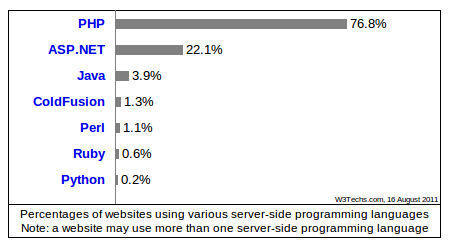
\includegraphics[scale=0.65]{images/Einleitung/serverseitigeScriptsprachen.png}
\caption{Nutzung verschiedener Programmiersprachen auf Servern}
\end{center}
\end{figure}

Auch im Bereich der Web Content Management Systeme\footnote{Im folgenden wird für den Begriff Web Content Management Systeme die Abkürzung WCMS verwendet} spiegelt sich diese Dominanz wider. Betrachtet man die Angaben des Content Management Portals cmsmatrix.org\footnote{\href{http://cmsmatrix.org}{http://cmsmatrix.org} ermöglicht eine Gegenüberstellung der Funktionalitäten von Content Management Systemen unterschiedlicher Prgrammiersprachen.}, existieren neben den vor allem in Deutschland verwendeten Open Source-Lösungen Typo3, Drupal, Contao oder Joomla! über 500 weitere in PHP implementierte Web Content Management Systeme unterschiedlichster Ausprägung und Qualität.
Ruby als Programmiersprache findet hingegen nur bei etwa 1 Prozent der erfassten Server Verwendung. Die dabei umgesetzten Projekte sind meist individuelle, browser-basierte Applikationen, die für Unternehmen und deren spezifisches Geschäftsfeld entwickelt wurden. Bekannte Vertreter sind hier u.a. die webbasierte Projektmanagement-Applikation Basecamp von 37signals\footnote{Projektseite von Basecamp:\href{http://basecamphq.com}{ http://basecamphq.com/}}, der Microblogging-Dienst Twitter\footnote{
Großteile der Programmierung von Twitter basierten bis April 2011 auf dem Ruby on Rails Framework.} und der webbasierte Hosting-Dienst Github\footnote{Github greift neben Ruby on Rails noch auf andere Webframeworks und Technologiesysteme zurück.
} für Software-Entwicklungsprojekte.
Diese individuellen Lösungen werden dabei meist unter Zuhilfenahme  eines Web Application Framework realisiert, das den Entwicklungsprozess unterstützt und vereinfacht.


%\begin{}
%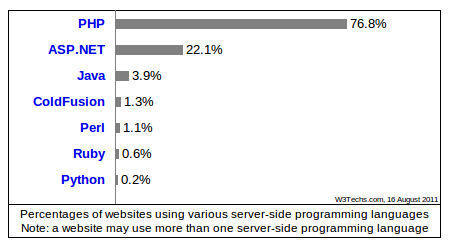
\includegraphics[width=\linewidth]{images/Einleitung/serverseitigeScriptsprachen.png}
%\caption{}
%\label{fig:beispiel}
%\end{figure}

\section{Motivation und Zielsetzung}

Ruby on Rails\footnote{Im weiteren Verlauf dieser Arbeit wird für das Webframework Ruby on Rails die Kurzform Rails verwendet.} hat sich seit der Veröffentlichung der Version 1.0 im Juli 2004 zu einem der bekanntesten Webframeworks der Ruby Fangemeinde entwickelt.
Startups\footnote{Der Begriff Startup bezeichnet hier junge Unternehmen, die sich mit ihrem neuartigen, meist innovativen Produkt noch nicht am Markt etabliert haben.} sowie etablierte Unternehmen greifen zunehmend auf das Rails Framework zurück, um ihre webbasierten Geschäftsideen und -modelle zu realisieren.
Wird neben der Webapplikation zusätzlich eine Internetseite zur Repräsentierung der Unternehmung benötigt, haben sich in der Praxis folgende zwei Lösungsansätze herausgebildet:

\begin{enumerate}
\item{
Bei geringem Umfang der zusätzlichen Internetseite werden die Inhalte manuell in HTML-Dateien angelegt und anschließend in die Rails-Anwendung integriert. Komfortable Möglichkeiten der Content-Verwaltung werden nicht angeboten oder später rudimentär nach implementiert. Änderungen der Inhalte sind teilweise mit erhöhtem Aufwand verbunden oder erfordern zusätzliche Programmierkenntnisse\footnote{Änderungen am Quellcode von Rails-Anwendungen im Produktivmodus erfordern immer einen Neustart des Servers.}.
}

\item{
Komplexe Internetseiten mit vielen Inhalten und anspruchsvollem Layout werden über ein Web Content Management System eines Drittanbieters realisiert. Die Rails-Anwendung fungiert als Zwischenstation und leitet bestimmte Anfragen an das externe WCMS weiter.
}
\end{enumerate}

Während der erste Lösungsansatz bei wenigen Inhalten noch vertretbar ist, erfordert die Verwendung eines externen WCMS zusätzlichen Installations- und Wartungsaufwand. Weiterhin erhöht sich der Bedarf an Programmierern, da neben Ruby nun auch andere Programmiersprachen Verwendung finden können.
\newline
\newline
Ziel der vorliegende Arbeit ist es daher, die Möglichkeiten einer komplett rails-basierten Web Content Management Verwaltung zu untersuchen, um so den Einsatz eines externen WCMS überflüssig werden zu lassen.
\newline
\newline
Dafür werden unter Verwendung der vergleichenden Methode die ausgewählten Ruby on Rails Content Management Systeme Alchemy CMS, Browser CMS, Locomotive CMS und Refinery CMS einem externen Kriterienkatalog gegenübergestellt, der allgemein gültige Anforderungen an Web Content Management Systeme formuliert. An Hand der Ergebnisse des Vergleichs kann abschließend eine Leistungsbeurteilung für die gewählten Systeme erfolgen und in wie weit sich diese für den Einsatz im Bereich des Webpublishing eignen.
Zusätzlich wird die programmiertechnische Umsetzung der Systeme analysiert und auf mögliche Probleme hingewiesen.

\section{Aufbau der Arbeit}
Die vorliegende Diplomarbeit gliedert sich in sechs wesentliche Abschnitte:
\newline
\newline
Im ersten Abschnitt, in Kapitel 2, werden die für die funktionelle und programmiertechnische Analyse der Systeme notwendigen theoretischen Grundlagen zu Web Content Management Systemen und dem Ruby on Rails Webframework geschaffen.
Darüber hinaus wird der für die Ermittlung der Leistungsfähigkeit der Systeme verwendete Kriterienkatalog vorgestellt.
\newline
\newline
Im zweiten Abschnitt, in Kapitel 3, folgt die funktionale Analyse der ausgewählten Ruby on Rails 3 Web Content Management Systeme Alchemy CMS, Refinery CMS, Browser CMS und Lokomotive CMS. Dazu werden die Kriterien des im Kapitel 2 vorgestellten Katalogs mit den tatsächlich gebotenen Funktionalitäten der gewählten WCMS verglichen. Die Untersuchung schließt mit einer Zusammenfassung der Ergebnisse und einer Einschätzung für den Einsatz der WCMS ab.\\
\newline
Kapitel 4 überprüft die analysierten WCM-Systeme auf vorhandene konzeptionelle und programmiertechnische Schwachstellen.
Darauf aufbauend werden in Kapitel 5 mögliche Lösungsansätze demonstriert und die dafür notwendigen theoretischen Grundlagen herausgearbeitet.
Kapitel 6 schließt die Arbeit mit einer Zusammenfassung der herausgearbeiteten Ergebnisse ab und gibt Ausblicke auf zukünftige Entwicklungspotenziale.
%
% EOF
%

